\documentclass[a4paper]{article}

\usepackage[T1]{fontenc}
\usepackage[margin=2.5cm]{geometry}
\usepackage{abstract}
\usepackage{url}
\usepackage{graphicx}

\author{The Unicorn Hunters\\
Christian Frantzen, Guilherme Barreiro Vieira,\\
Mortimer Sotom and Théo Verhelst}
\title{Advanced Machine Learning Coursework: Kaggle Competition NYC Taxis}

\begin{document}
\maketitle


\begin{abstract}
Accurate prediction of taxi trip duration is an important part of efficient
customer service for taxi companies. To this end, the New York City Taxi
and Limousine Commission organised a competition on the Kaggle website, aiming
to stimulate research in taxi trip duration regression. This report presents the
work that our team conducted on this problem. A classical machine learning
pipeline has been applied: data analysis, data cleaning, feature selection,
model evaluation and optimisation. The models that have been tried range from
Ridge Regression to Extreme Gradient Boosting. An unlabeled test set is proposed
to the competitors in order to accurately evaluate the generalisation
performance of their models. The predictions of our best models on this test set
gave us a decent ranking in the top 20\% of the competition leaderboard.
\end{abstract}

\section{Introduction}
New York City (NYC) is one of the busiest cities in the world with pedestrians
constantly rushing to arrive to their destination on time. To avoid searching
for parking and the stress of driving during rush hour, most citizens of NYC use
public transport, and especially taxis. The most important piece of information
is undoubtedly the estimated trip duration for customers to plan their schedule,
for the driver to find the shortest route and for deriving the estimated price
of the journey. This is exactly the aim of the ``New York City Taxi Trip
Duration'' Kaggle competition, build a model able to predict the total ride
duration of taxi trips given a set of features such as geo-coordinates, number
of passengers and others. The dataset provided is one released by the NYC Taxi
and Limousine Commission (TLC) and contains over 1.45 million trip records over
the entire year of 2016. Participants must then predict the trip duration in
seconds for each entry of the test set containing 625,134 trip records.

Before diving into building predictive models, the data must be carefully
analysed to gain an understanding of the features provided and the problem at
hand. The next was preprocessing the data and augmenting it with hourly
rainfall, further distance measurements and road related informations from The
Open Source Routing Machine (ORSM). Section four explains how the relevance of
each feature was evaluated by information gain and recursive feature selection.
The following section describes the chosen evaluation metric, Root Mean Squared
Logarithmic Error (RMSLE), and the reasoning behind also predicting the trip
durations in minutes by classification. Finally, a total of seven models were
implemented: Adaboost, Support Vector Machine (SVM), Gaussian Process,
Stochastic Gradient Descent, Random Forest, Extreme Gradient Boosting (XGBoost)
and Neural Network (NN). The results of each model is presented and discussed in
the last section of this report.


\section{Data Analysis}
The first step of a machine learning project is to explore and analyse the data,
in order to better understand the problem. Our dataset is composed of 11
features: a unique identifier for each row, the identifier of the taxi company,
the pickup time, the pickup and drop-off locations, the number of passengers,
and a boolean flag indicated if the trip data has been stored on-board or
directly sent to the data server.

Figures \ref{long} to \ref{pickup_hour} show the distribution of some of these
features. Pickup month, minute and seconds are not shown, as their graphs
are uniformly distributed and therefore not visually informative. Outliers have
been removed in order to properly display the pickup and drop-off location
distribution, as well as the trip duration. These outliers will be discussed in
the next section. One can see in figure \ref{long} and \ref{lat} that the
location seems to be roughly normally distributed, and the logarithm of the trip
duration also appears to be normally distributed in figure
\ref{log_trip_duration}. The smaller bumps outside of the main bell in the
location curves correspond to trips to the two city airports.

\begin{figure}
    \centering
   \begin{minipage}{.45\textwidth}
        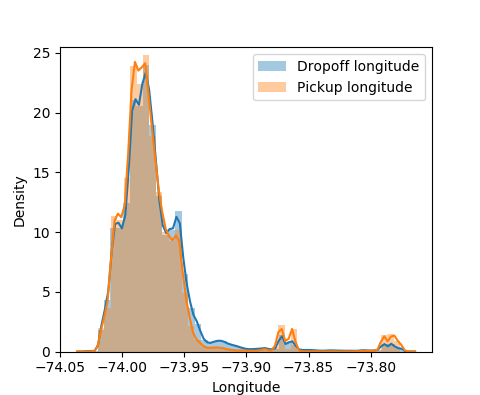
\includegraphics[width=\linewidth]{longitude}
        \caption{Distribtion of the longitude.}
        \label{long}
    \end{minipage}
    \hspace{0.05\textwidth}
    \begin{minipage}{.45\textwidth}
        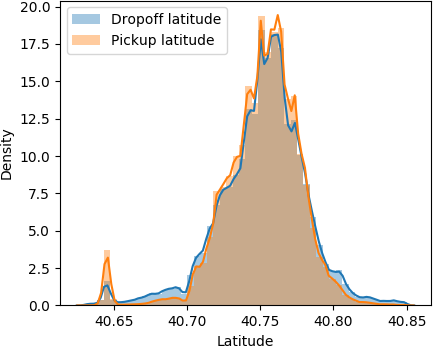
\includegraphics[width=\linewidth]{latitude}
        \caption{Distribution of the latitude.}
        \label{lat}
    \end{minipage}
\end{figure}

\begin{figure}
    \centering
    \begin{minipage}{.45\textwidth}
        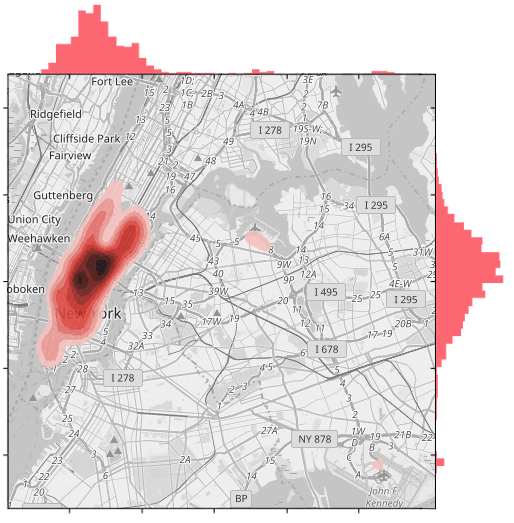
\includegraphics[width=\linewidth]{map_kde}
        \caption{Heatmap of the trip locations on a map (credits: OpenStreetMap).}
        \label{heatmap}
    \end{minipage}
    \hspace{0.05\textwidth}
   \begin{minipage}{.45\textwidth}
       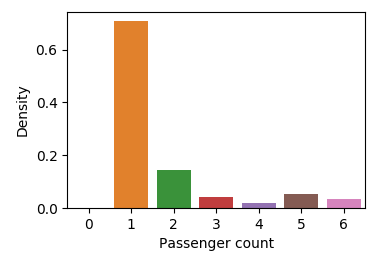
\includegraphics[width=\linewidth]{passenger_count}
       \caption{Distribution of the number of passengers.}
       \label{passenger_count}
    \end{minipage}
\end{figure}

\begin{figure}
    \centering
    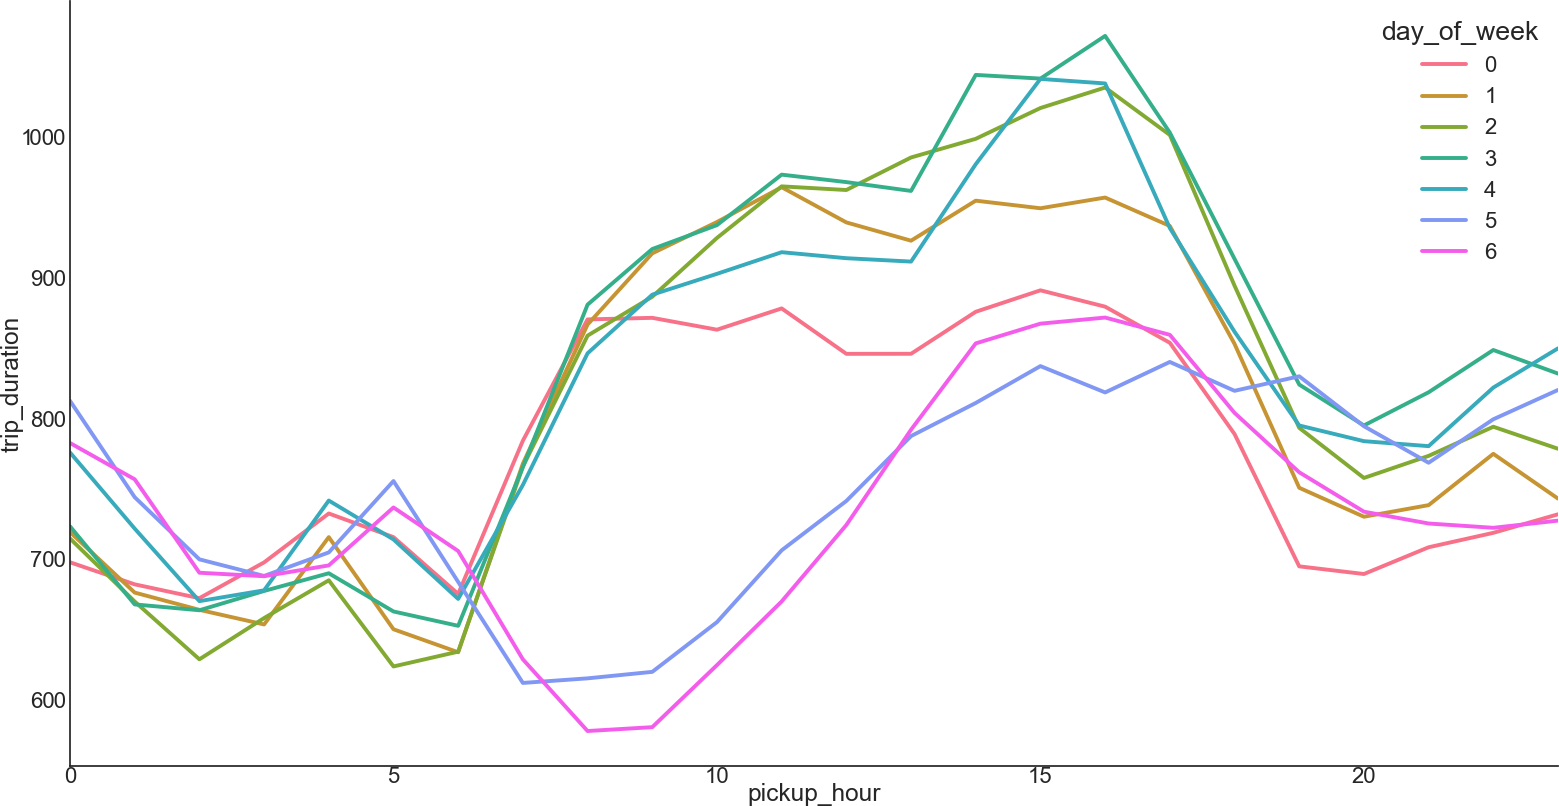
\includegraphics[width=\linewidth]{pickup_hour_vs_trip_duration}
    \caption{Distribution of the pickup time, for different days of the week.}
    \label{pickup_hour}
\end{figure}

\begin{figure}
    \centering
    \begin{minipage}{.45\textwidth}
        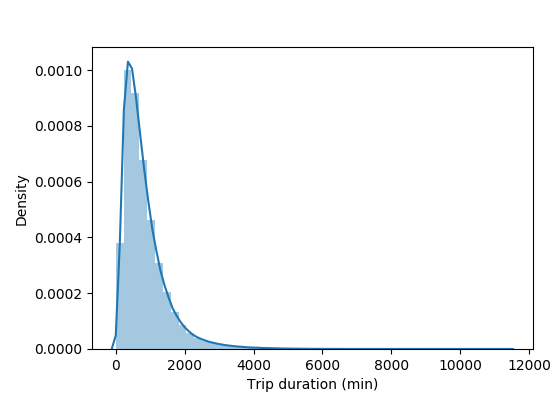
\includegraphics[width=\linewidth]{trip_duration}
        \caption{Distribution of the trip duration, in seconds.}
        \label{trip_duration}
    \end{minipage}
    \hspace{0.05\textwidth}
   \begin{minipage}{.45\textwidth}
       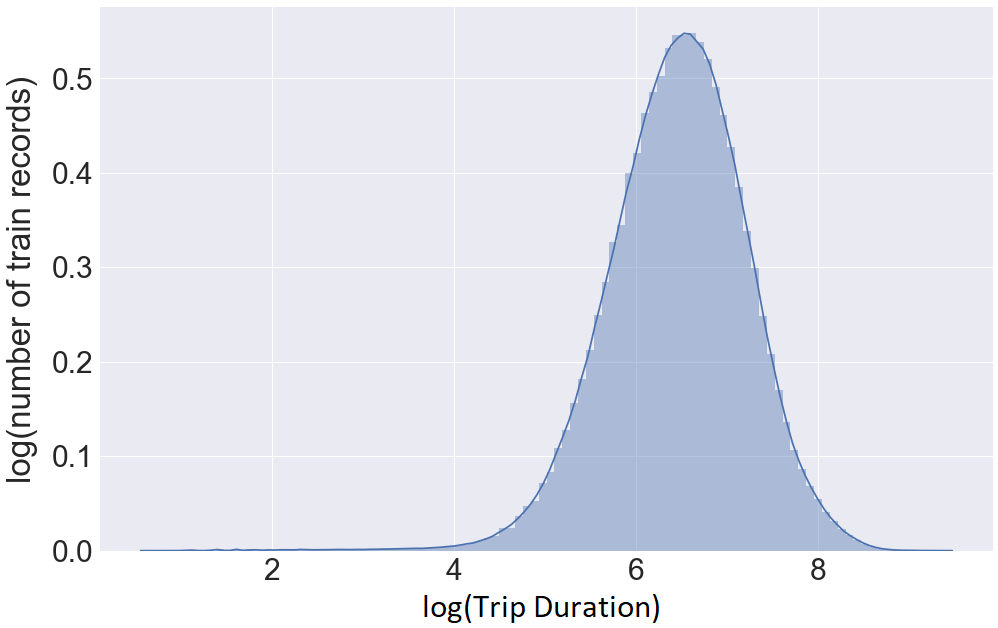
\includegraphics[width=\linewidth]{log_trip_duration}
       \caption{Distribution of the logarithm of the trip duration, in seconds.}
       \label{log_trip_duration}
    \end{minipage}
\end{figure}

It is also important to make sure that the training and test sets are
independently and identically distributed. For this, the above distributions
have been compared with those from the test set. If the distribution from the
training and testing set significantly overlap, then it can be supposed that
the I.I.D. assumption is verified. As shown for example in figure
\ref{test_vs_train_long} and \ref{test_vs_train_lat}, it is indeed the case.

\begin{figure}
    \centering
    \begin{minipage}{.45\textwidth}
        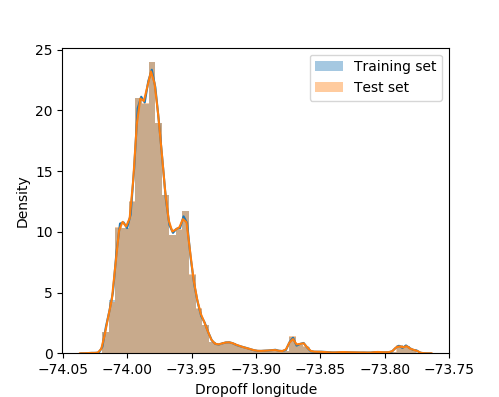
\includegraphics[width=\linewidth]{test_vs_train_long}
        \caption{Drop-off longitude in the training and test set.}
        \label{test_vs_train_long}
    \end{minipage}
    \hspace{0.05\textwidth}
   \begin{minipage}{.45\textwidth}
       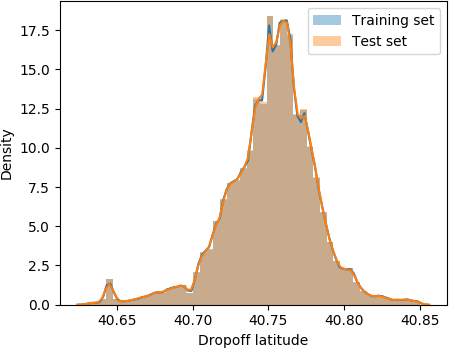
\includegraphics[width=\linewidth]{test_vs_train_lat}
       \caption{Drop-off latitude in the training and test set.}
       \label{test_vs_train_lat}
    \end{minipage}
\end{figure}

\section{Preprocessing}
Since the data is provided by Kaggle, it is already very clean. However, when
looking at the distributions of the GPS coordinates and the trip durations, we
observed that some trips were outliers. We calculated the mean value for the
trip duration (961 seconds) and the standard deviation (5247 seconds) and then
removed all trips which were shorter than the mean minus twice the standard
deviation or longer than the mean + twice the standard deviation. We also
removed all trips which were not in the following bounds for their coordinates :
longitude $[-74.03;-73.77]$ and latitude : $[40.63;40.85]$.

To augment our  dataset  we downloaded weather data from 2016 from IEM Computed
Hourly Precipitation Totals by Iowa State University
(\url{https://mesonet.agron.iastate.edu/request/asos/hourlyprecip.phtml?network=NY_ASOS})
and extracted the volume of precipitation for each of our trips. Next, we used
the GPS coordinates of the pickup and drop-off locations to calculate following
properties:
\begin{itemize}
    \item Distance between the two points curved along the surface of the
earth called, Vincenty's distance;
    \item Pythagorean distance between the two points;
    \item Manhattan distance;
    \item The angle between the two points in relation to the north pole, called bearing.
\end{itemize}
We also used OSRM (\url{http://project-osrm.org/}) to give us information
about the cab ride. OSRM stands for open source routing machine and makes it
possible to download maps from all around the world and calculate the street
distance between two points as well as other information. Besides the street
distance, the number of turns to make before reaching the
destination has been included, as well as how many intersections one has to pass.  Apart from the data
provided by Kaggle we could also have used more trip records available on the
website of the NYC Taxi and Limousine Commission. However the files available
are of the size of a few gigabytes per month, which is why decided not to
include them.

Additionally to the data augmentation we also always scale it before passing it to a model. Sklearn provides the possibility to center every column to the mean and scale to unit variance.

\section{Feature Selection}
In order to ensure that the model was not being fed useless features, a feature
selection elimination procedure was undertaken. The results are shown in the
above figure - the lower the ranking the better the feature is - by using the
scikit-learn package recursive feature elimination. This function attempted to
find a ranking of the features by doing a prediction while removing one feature
at the time. As expected the most important features such as drop-off and pickup
locations as well as different measures of distance were ranked as very
important. In contrast,  features that didn’t contain much information such as
\texttt{pickup\_year}, \texttt{store\_and\_fwd\_flag}, \texttt{vendor\_id} and
\texttt{pickup\_month}, were ranked as very low importance and hence were
removed from the model. Interestingly enough, the precipitation feature
providing an idea of the weather conditions, didn’t rank very low leading to
believe that it didn’t have a significant effect in the duration of the trips
within New York and specifically Manhattan which is where most of the journeys
were recorded.

\begin{figure}
    \centering
    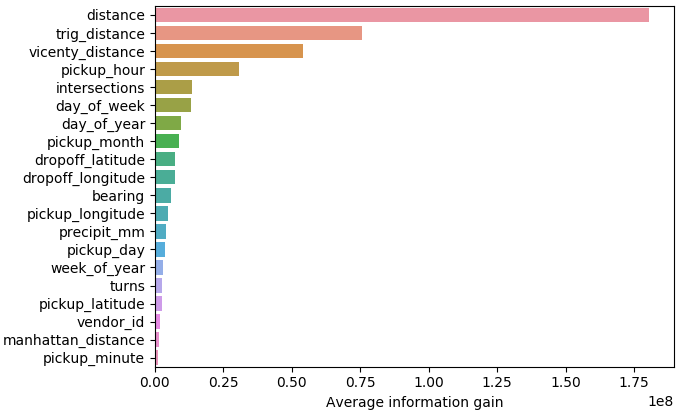
\includegraphics[width=0.8\linewidth]{feature_importance_seaborn}
    \caption{Information gain of each feature.}
    \label{information_gain}
\end{figure}

On the other hand an analysis of feature importance in figure \ref{information_gain} provides
a different perspective on which features provide more information gain to the
model. It is expected that the distances add the most significant amount of
information with exception of the Manhattan distance which apparently adds
little information - contradicting the RFE analysis. Furthermore, the amount of
intersections, day of the week and day of the year have significant amount more
value to the model than previously. This is a good indication of the different
amount of congestion at different times of week and year whereas in this
analysis it seems that the coordinate locations add less value as they change
less due to being majorly close by within the city. Finally, note that some of
the features within this information gain analysis have been removed from the
last one, however, by removing any more features within this selection, the
models error increased, hence, this selection of features was chosen as the
final one.

\section{Methods for Model Selection}
In order to assess the performance of each model to be tested and compare the
results, an error metric was selected. To remain consistent with the scoring of
the Kaggle competition, the same evaluation function was chosen: Root Mean
Squared Logarithmic Error (RMSLE). This allows to estimate the leaderboard
ranking of the results and since it is logarithmic, it ensures that the
prediction for short trips have the same weighting as the predictions for long
trips. The RMSLE is calculated as

\[RMSLE = \sqrt{\frac{1}{n}\sum_{i=1}^n(\log(p_i+1) - \log(a_i+1))^2}\]

Where $n$ is the total number of entries in the data set, $p_i$ is the predicted trip
duration and $a_i$ is the true trip duration.  The dummy regressor was implemented
to use as a benchmark since its predictions employ basic rules, to further
compare the regression models. It achieved a high RMSLE of 0.810 for the
prediction in seconds and 0.802 for the prediction in minutes.  Additionally to
predicting the trip duration in seconds through regression, each model was
designed to predict the trip duration in minutes through classification for a
more logical and interpretable estimate. In real life scenarios, it would be
unrealistic to predict a taxi journey to the exact second due to the dynamic
environment of the city.

\section{Results}
As previously mentioned, the results of each model will be presented in terms of
their RMSLE score and the predictions in minutes through classification. The
final optimised results of all models can observed and compared in table
\ref{results}. Each model was initially tested by running with the default
parameters and it became evident that neural networks, random forest and XGBoost
performed much better than the remaining models. Those three models were
extensively tested and optimised with all data available in appendix
\ref{results_appendix}. A grid search was still applied to the less performant
models but no further time was invested in optimising them since it was evident
they would not outperform the top three models and hence the lack of testing
results in the appendix.

\subsection{Extreme Gradient Boosting}
Since this problem uses a relatively large dataset, it was expected that Extreme
Gradient Boosting (XGBoost) would perform well. Using the default parameter
values and all of the available features, it produced a baseline score of 0.394.
After applying grid search to optimise the hyper-parameters (see appendix
\ref{results_appendix}) and removing features suggested by the feature selection
elimination, the RMSLE was reduced to 0.346, making XGBoost perform slightly
better than NN and becoming the best tested model. $l_1$ and $l_2$
regularisation terms were also introduced in an attempt to further improve the
prediction accuracy but regardless of the values used, no effect could be
observed. While training the model, an internal parameter controls which metric
is used to calculate the evaluation for validation data. Unfortunately, no
customised function can be passed so the RMSE was used but it is believed that
if this parameter was customisable, using RMSLE as an error metric would
marginally improve the results.


\subsection{Neural Networks}
Neural networks (NN) performed well in this data set with some hyper-parameters
tuning. At first, due to the nonlinearity of the data, models with up to 3
hidden layers and 512 nodes were experimented on, however, the results were far
from satisfactory. As one tried to reduce the complexity of the model, in which
the optimum point was found to be with three layers of 64 nodes - errors reduced
down to around 0.35 RMSLE. Following this, hyper-parameters grid search such as
the type of solver, activation function, batch size and amount of regularisation
were conducted which led to finding our optimal model. The Adam solver was the
most efficient which was expected as it is a good solver for large datasets,
with a relu activation function, some regularisation and small batch sizes of
200, which brought the error down to 0.346.

\subsection{Random Forest}
Random forest builds multiple decision trees and merges them together to get a
more accurate and stable prediction. This algorithm proved to be a powerful
algorithm for this dataset as it brings an extra aspect of randomness into the
model, as when it is growing the trees, it searches for the best feature among a
random subset of features instead of searching for the best feature while
splitting a node. This increases the diversity of the model which in this case
resulted in better results. The key hyper-parameters in this model were the
number of estimators (number of trees in the forest), the minimum number of
samples required to split a node and the minimum number of samples required to
be at a leaf node. The prediction error was always reduced by the number of
estimators of which it was increased up to the hardware memory capability - 125
estimators which led to an error of 0.36. On the other hand, the other
parameters were more finely tuned to reach the conclusion that the lower the
number of minimum samples split and minimum samples leaf, the higher the
overfitting likelihood within the model. Hence, by increasing these parameters,
an optimum error value was found to be at 0.346 thereby reaching one of the most
performant models within the trials conducted.

\subsection{Support Vector Machine}
The power of Support Vector Machine (SVM) is appealing, given its low
generalisation error. However, the time complexity of the training phase of the
SVM is proportional to the cube of the number of training examples, and as a
result it is impossible to train on our entire dataset, which is composed of
more than 1,400,000 samples. Therefore, a SVM regressor has been trained on a
random subset of the training set, which would contain up to 20,000 random
samples. Past this value, the training time is simply unbearable.

On the other hand, since the evaluation of a trained SVM model is fast, it was
possible to validate the model on a larger portion of the training set, thus
giving a strong estimation of the generalisation performance. It turns out that
by training a SVM on 20,000 samples, testing it on 100,000 samples and with a
suitable hyper-parameter optimisation, a SVM model achieves a RSMLE of 0.359.

\subsection{Stochastic Gradient Descent}
Using the Stochastic Gradient Descent regressor from sklearn, we got an RMSLE of
0.487 without any hyper-parameter tuning. Using grid search however we managed to
achieve an RMSLE of around 0.455. While we do scale our features before running
the model, it does not seem to get closer to the true objective function. This
may be due to the nature of GPS coordinates which are difficult to linearise.

\subsection{Gaussian Process}
Just as the support vector machine, the Gaussian Process (GP) has a time
complexity of $O(n^3)$. Therefore, it was unbearable to train a GP model with
the whole dataset. After a grid search to find the optimal hyper-parameters, a
GP model has been trained with a rational quadratic kernel, and a noise
reduction parameter $\alpha=0.01$, on 1000 random samples and then validated on
100,000 other samples. The RSMLE was calculated to be 0.469, which is most
probably due to underfitting, due to the very limited number of training
samples.

\begin{table}[h!]
    \centering
    \begin{tabular}{ccc}
        Model & RMSLE regression & RMSLE classification\\
        \hline
        XGBoost & 0.346 & 0.286 \\
        Neural Network & 0.347 & 0.136 \\
        Random Forest & 0.350 & 0.312 \\
        SVM & 0.359 & NA \\
        SGD & 0.475 & 0.400 \\
        Gaussian Process & 0.512 & 0.500 \\
        Ridge Regression & 0.539 & NA \\
        Dummy Regressor & 0.810 & 0.802 \\
        AdaBoost & 0.990 & 0.800 \\
        \hline
    \end{tabular}
    \caption{Comparison of the RMLSE of all tried models.}
    \label{results}
\end{table}

\section{Conclusion}
As our first real team machine learning project, we tackled this introductory
Kaggle competition with a lot of curiosity. Having enriched the provided data
significantly with help from OSRM we managed to establish a decent model with
Extreme Gradient Boosting, which ranks us XX on the Kaggle competition
leaderboard. While we did improve the data set we could have gone further by
including the available files on the NYC TLC’s website the increase the number
of samples, just as using a sophisticated way of linearizing GPS coordinates
like one-hot encoding could have helped the improve the predictions. This could
be studied in a next Kaggle competition using this kind of data. For the time
being, we can be be happy with what we learned in the process and look forward
to our next challenges as machine learners.

\newpage
\footnotesize
\bibliographystyle{ieeetr}
\bibliography{report}

\appendix
\newpage
\section{Additional Figures}
\begin{figure}[h!]
    \centering
    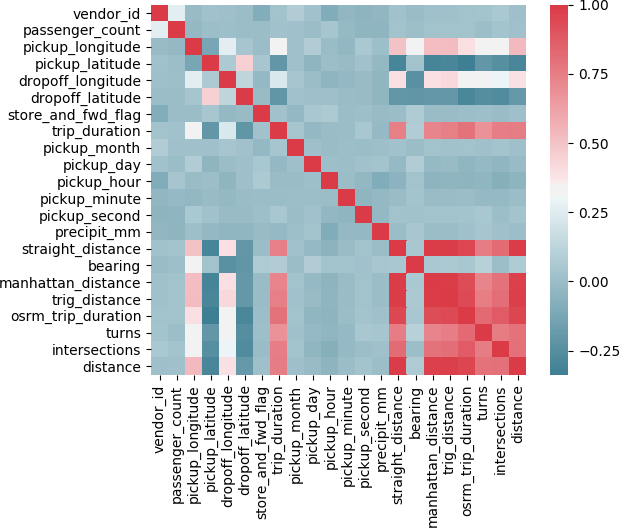
\includegraphics[width=0.8\linewidth]{confusion}
    \caption{Confusion matrix of the extended dataset.}
    \label{confusion}
\end{figure}

\section{Detailled Grid Search results}
\label{results_appendix}

\end{document}
